% uncertainties in tki_coplanar xsecs
\subsection{Supplemental:  Uncertainties in Cross Sections and Ratios} 
\label{sec:appendixB}
The uncertainties on the absolute cross sections and cross-section ratios to scintillator (CH) as a function of all the kinematic variables besides described in the main body of the paper (except \tkidelta\ ) are presented in this Appendix.  The format for each figure is the same:  the top five plots show the uncertainties on the absolute cross sections for CH, carbon, water, iron and lead.  Note that because the statistical uncertainties in carbon and water are large compared to the other targets, those uncertainties have been scaled by 0.5 to be plotted next to the uncertainties on the CH target.  The bottom four plots show the uncertainties in the ratios of the absolute cross sections to CH.  Note that the flux and muon reconstruction uncertainties largely cancel in the ratio, and the statistical uncertainty in the ratio is close to that of the absolute cross sections due to the large mass of the scintillator (CH) target compared to the passive targets.  
\begin{figure}
	\centering
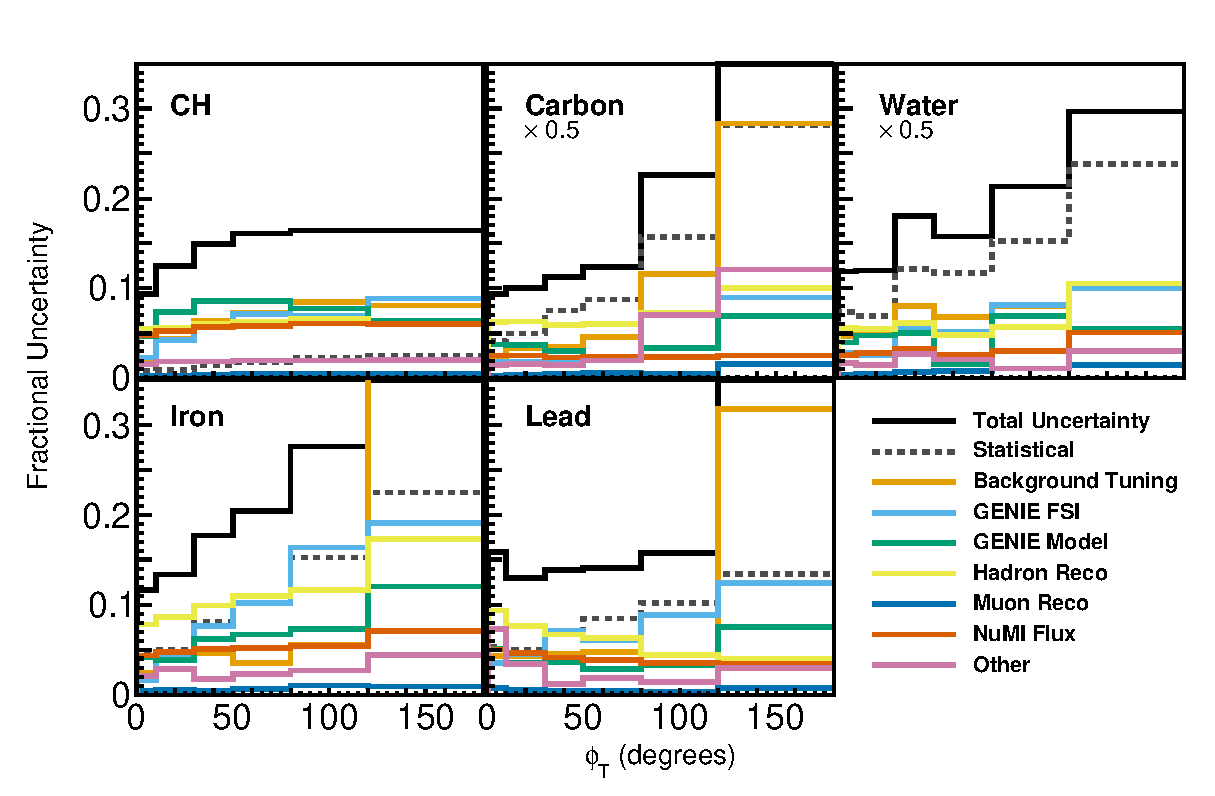
\includegraphics[width=\linewidth]{Figures/xsec_errors_all5/errors_phi.eps}
    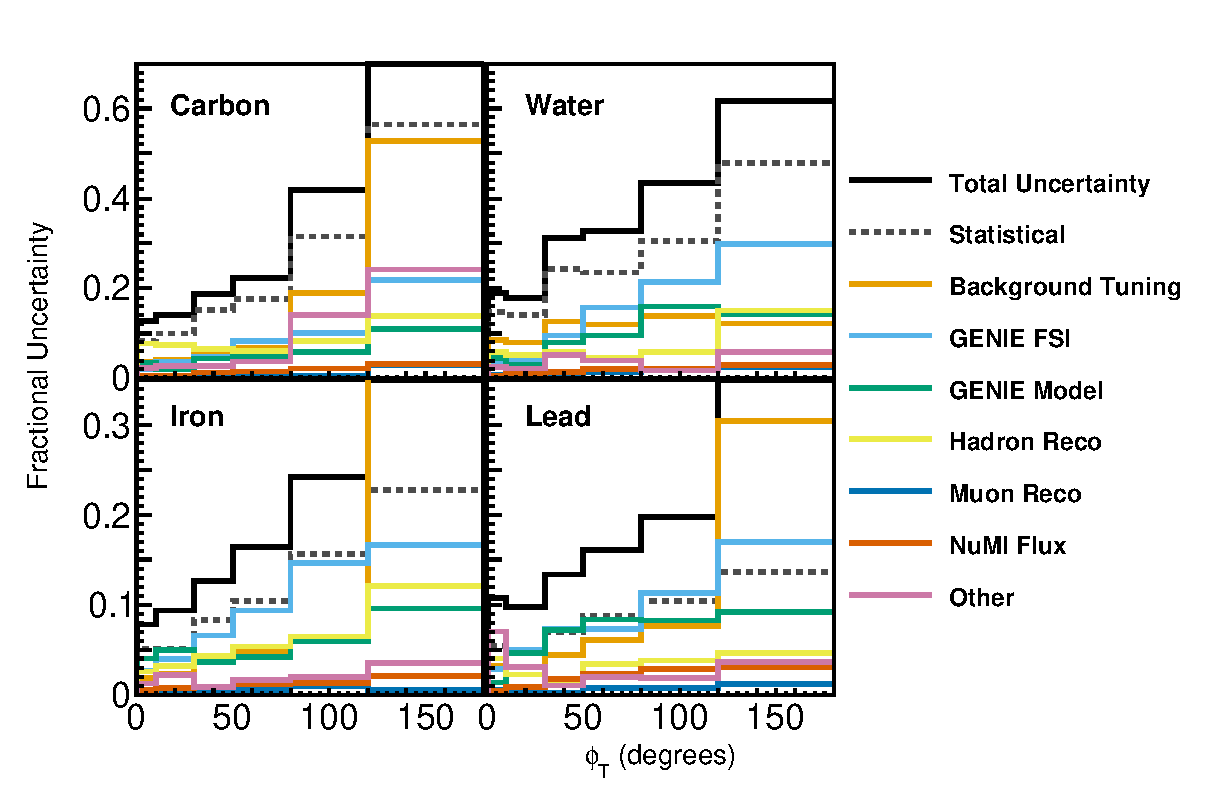
\includegraphics[width=\linewidth]{Figures/xsec_ratio_errors/ratio_errors_phi.eps}
    \caption[\tkicoplanar cross-section uncertainties for multiple targets]{Uncertainties on the absolute cross section for each target (upper five plots) and on the ratio to CH (lower four plots) for \tkicoplanar.}
    \label{fig:xsec_err_coplan}
\end{figure}
% uncertainties in tki_alpha xsecs
%
%  alpha
%
\begin{figure}
	\centering
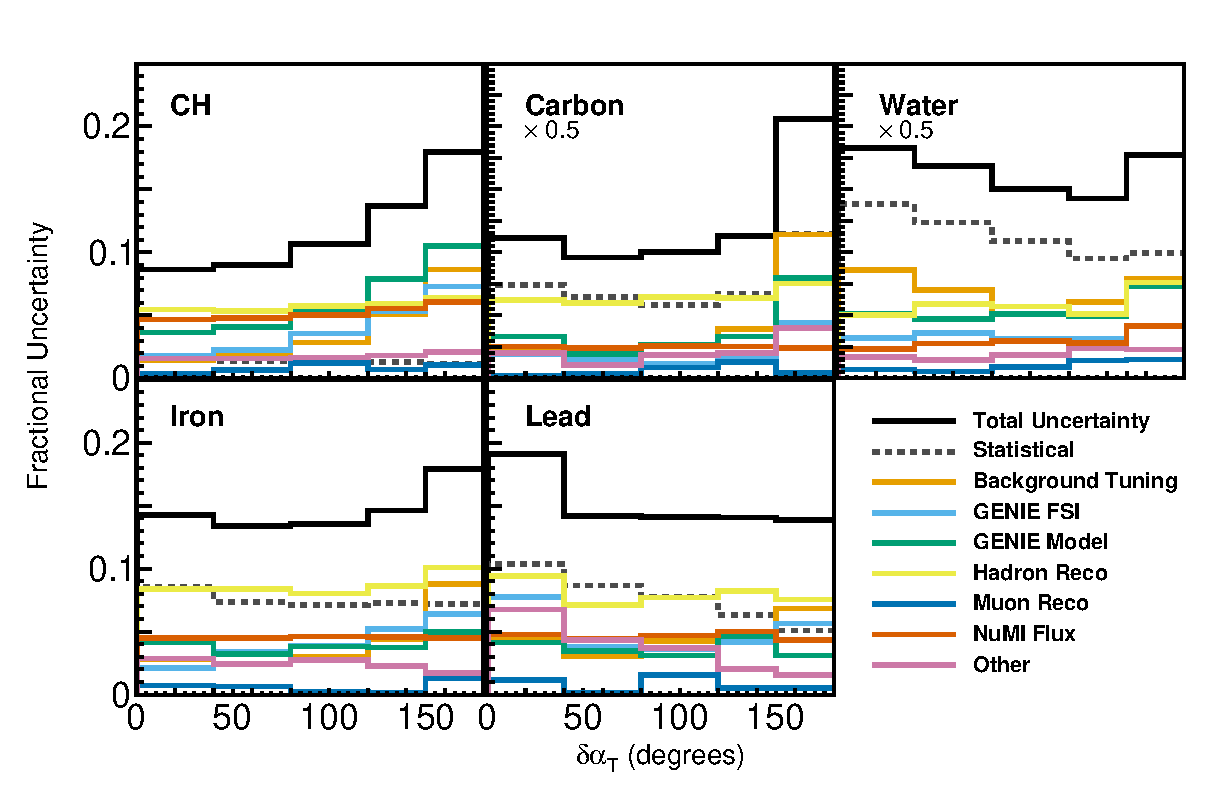
\includegraphics[width=\linewidth]{Figures/xsec_errors_all5/errors_alpha.eps}
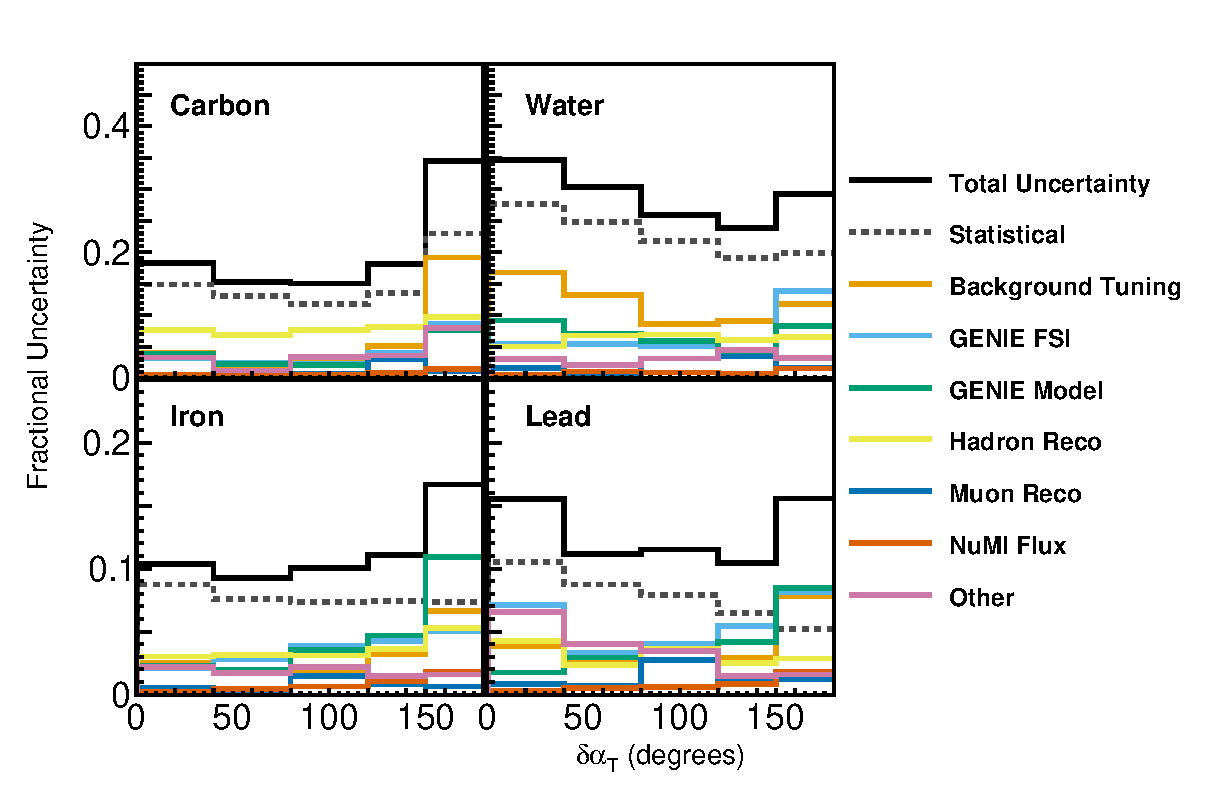
\includegraphics[width=\linewidth]{Figures/xsec_ratio_errors/ratio_errors_alpha.eps}
    \caption[\tkialpha cross-section uncertainties for multiple targets]{Uncertainties on the absolute cross section for each target (upper five plots) and on the ratio to CH (lower four plots) for \tkialpha.}
    \label{fig:xsec_err_alpha}
\end{figure}
% dptx
\begin{figure}
	\centering
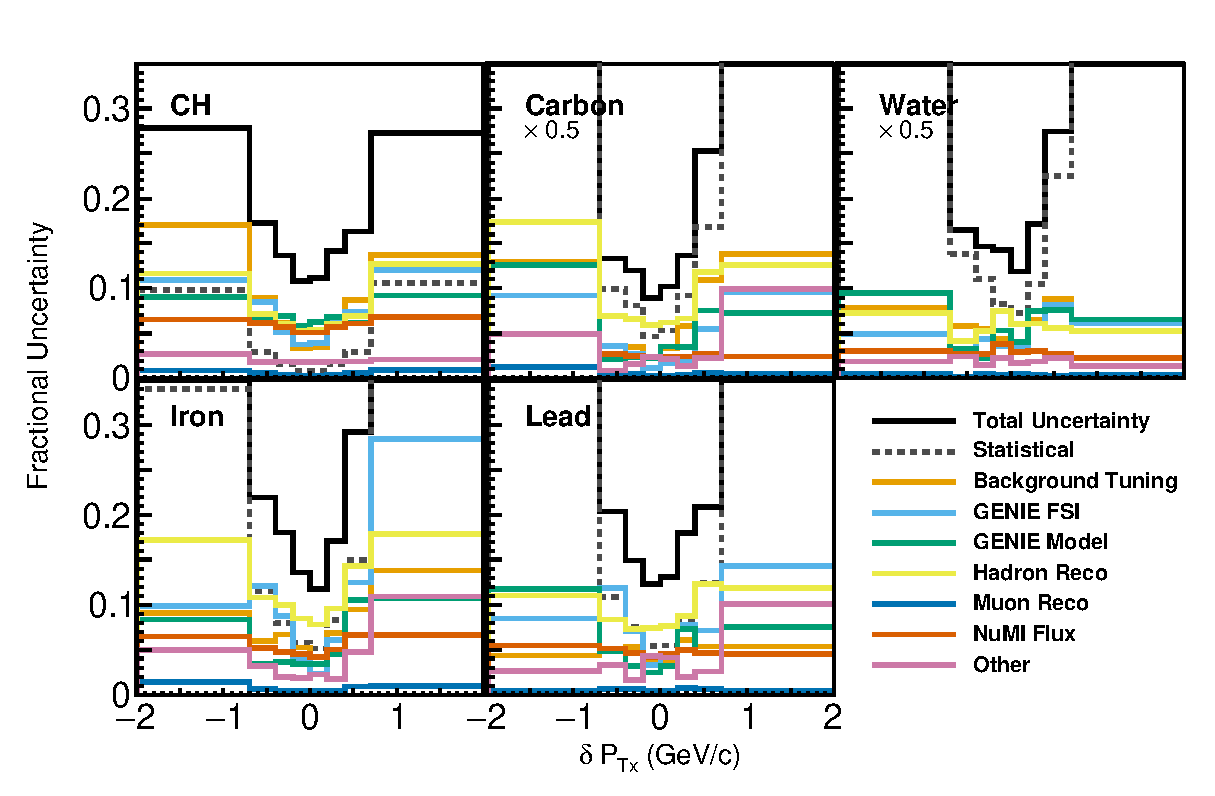
\includegraphics[width=\linewidth]{Figures/xsec_errors_all5/errors_dptx.eps}
    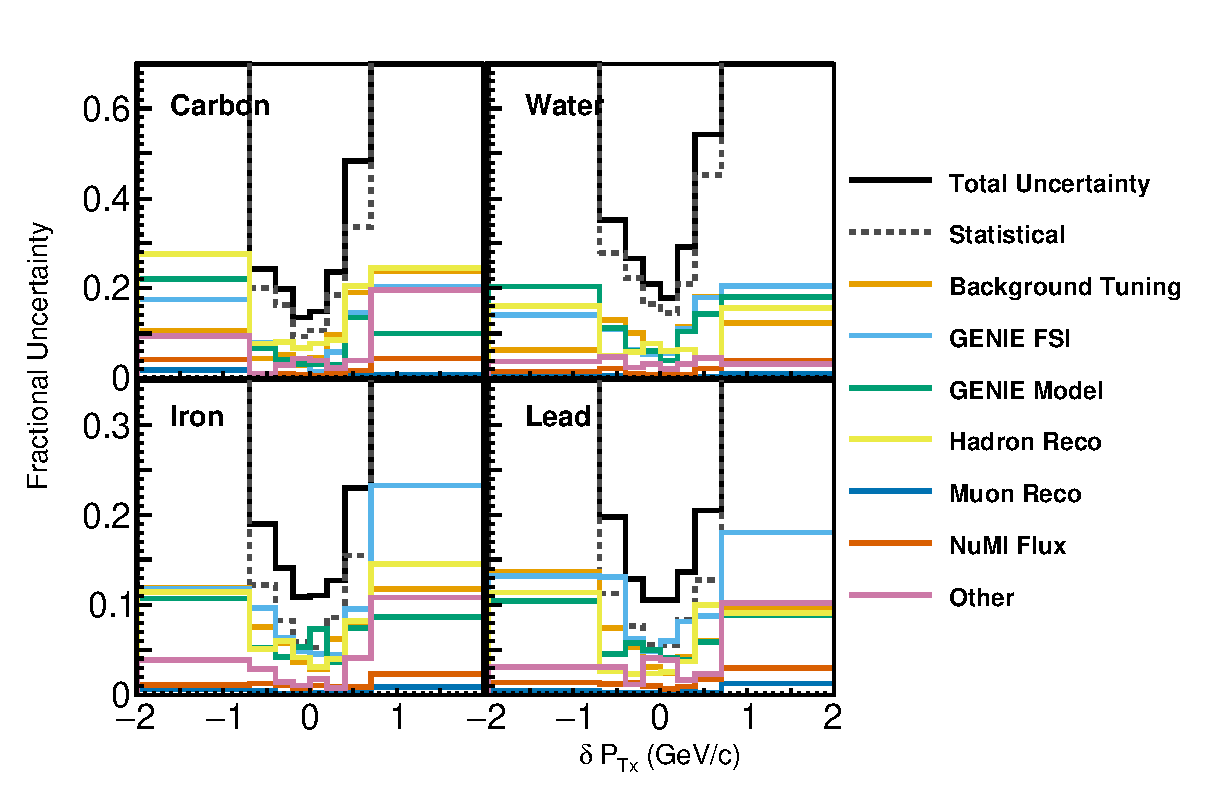
\includegraphics[width=\linewidth]{Figures/xsec_ratio_errors/ratio_errors_dptx.eps}
    \caption[\tkidptx cross-section uncertainties for multiple targets]{Uncertainties on the absolute cross section for each target (upper five plots) and on the ratio to CH (lower four plots) as a function of \tkidptx.}
    \label{fig:xsec_err_dptx}
\end{figure}
% dpty
\begin{figure}
	\centering
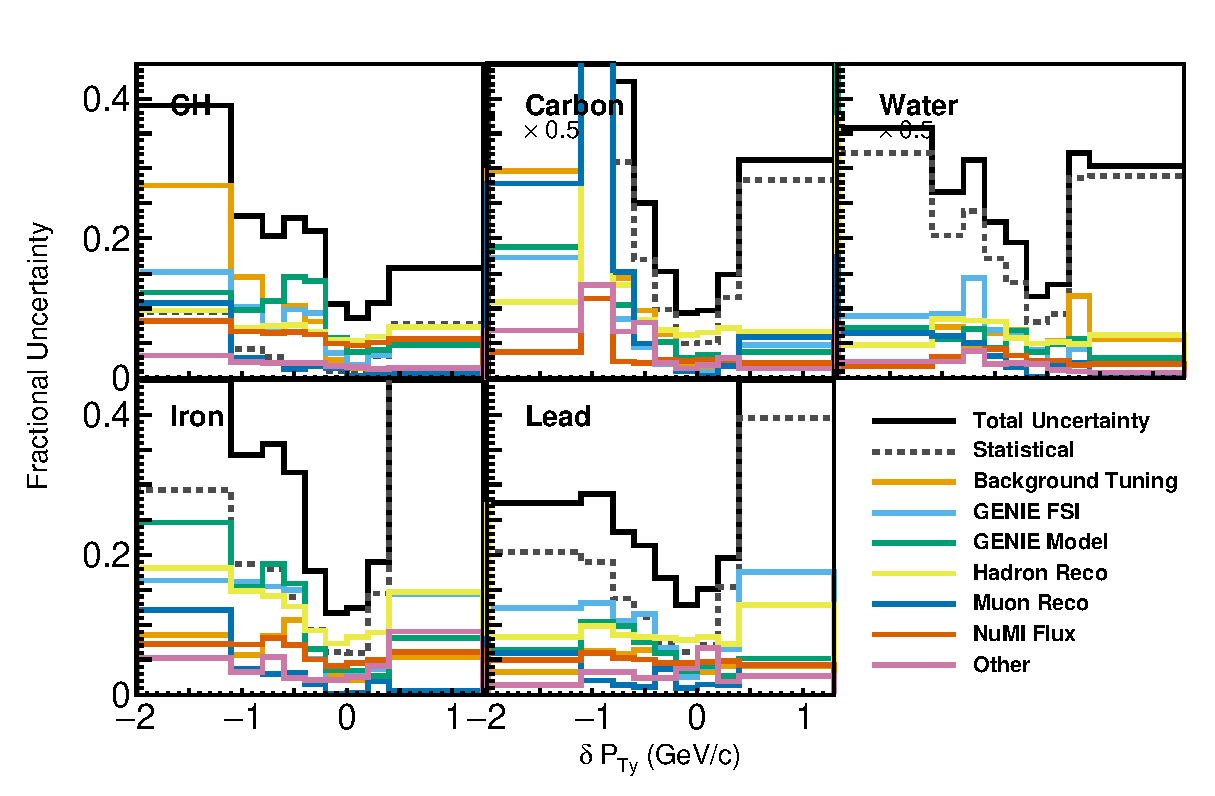
\includegraphics[width=\linewidth]{Figures/xsec_errors_all5/errors_dpty.eps}
    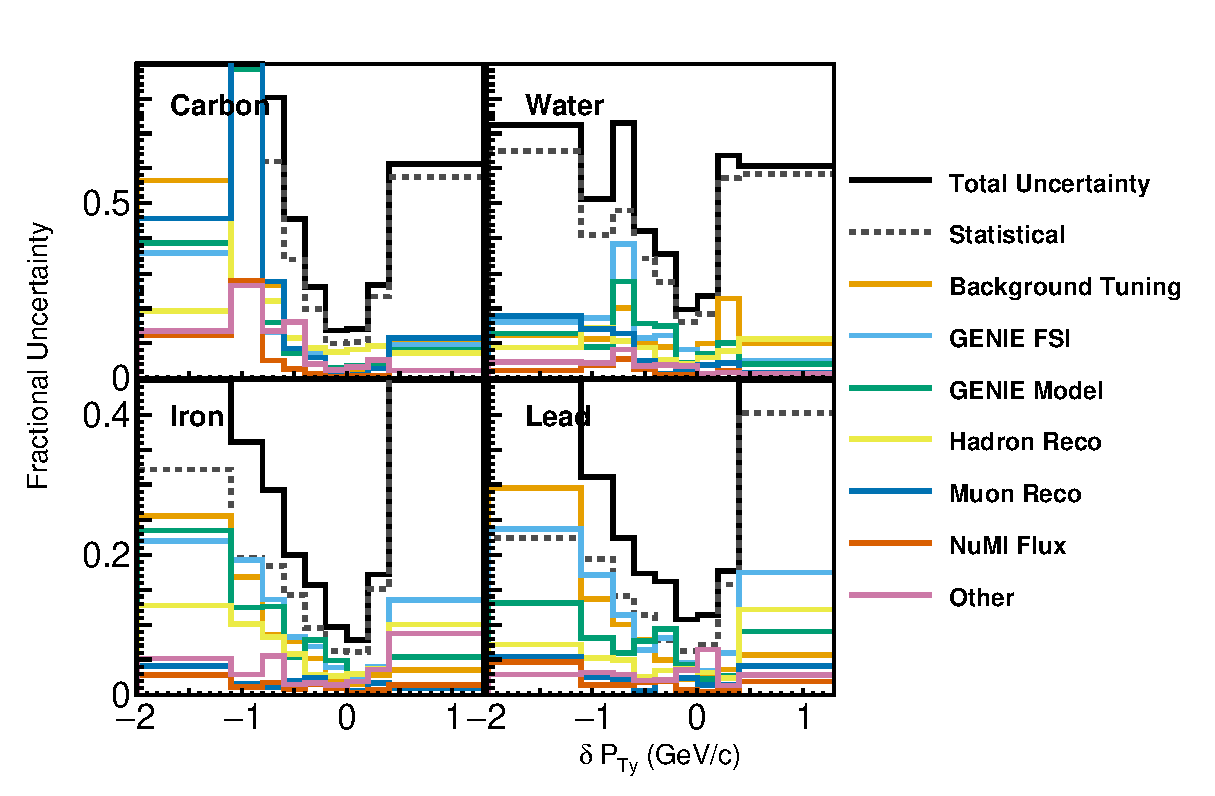
\includegraphics[width=\linewidth]{Figures/xsec_ratio_errors/ratio_errors_dpty.eps}
    \caption[\tkidpty cross-section uncertainties for multiple target ratios]{Uncertainties on the absolute cross section for each target (upper five plots) and on the ratio to CH (lower four plots) as a function of \tkidpty.}
    \label{fig:xsec_err_dpty}
\end{figure}
% dpl
\begin{figure}
	\centering
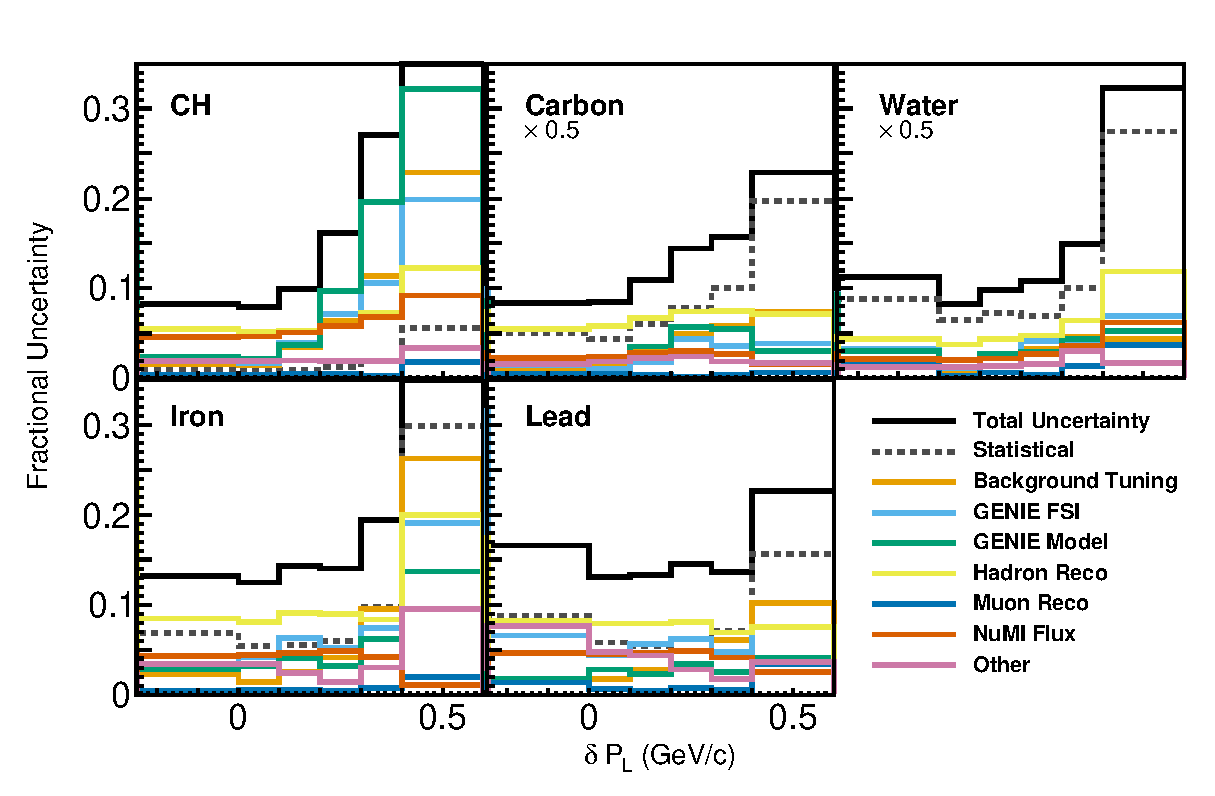
\includegraphics[width=\linewidth]{Figures/xsec_errors_all5/errors_pl.eps}
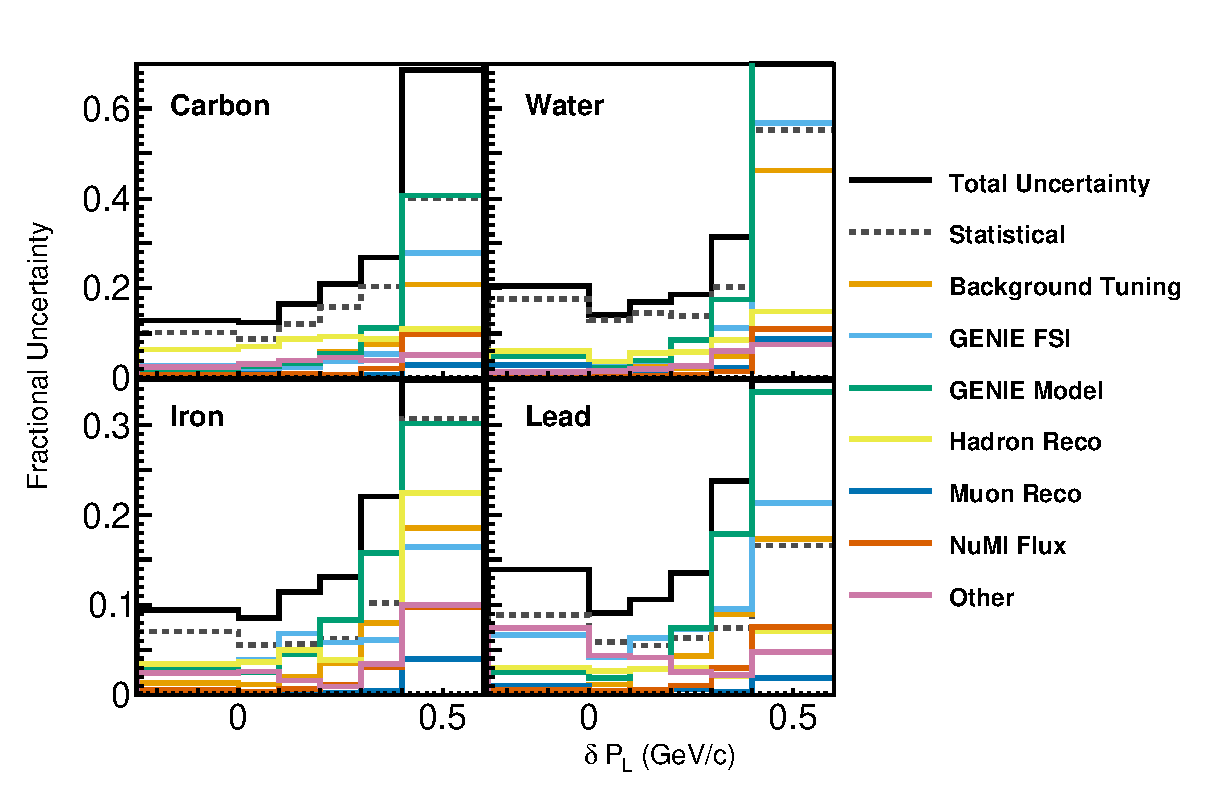
\includegraphics[width=\linewidth]{Figures/xsec_ratio_errors/ratio_errors_pl.eps}    \caption[\tkipl cross-section uncertainties for multiple targets]{Uncertainties on the absolute cross section for each target (upper five plots) and on the ratio to CH (lower four plots) as a function of \tkipl.}
    \label{fig:xsec_err_pl}
\end{figure}
% pn
\begin{figure}
	\centering
    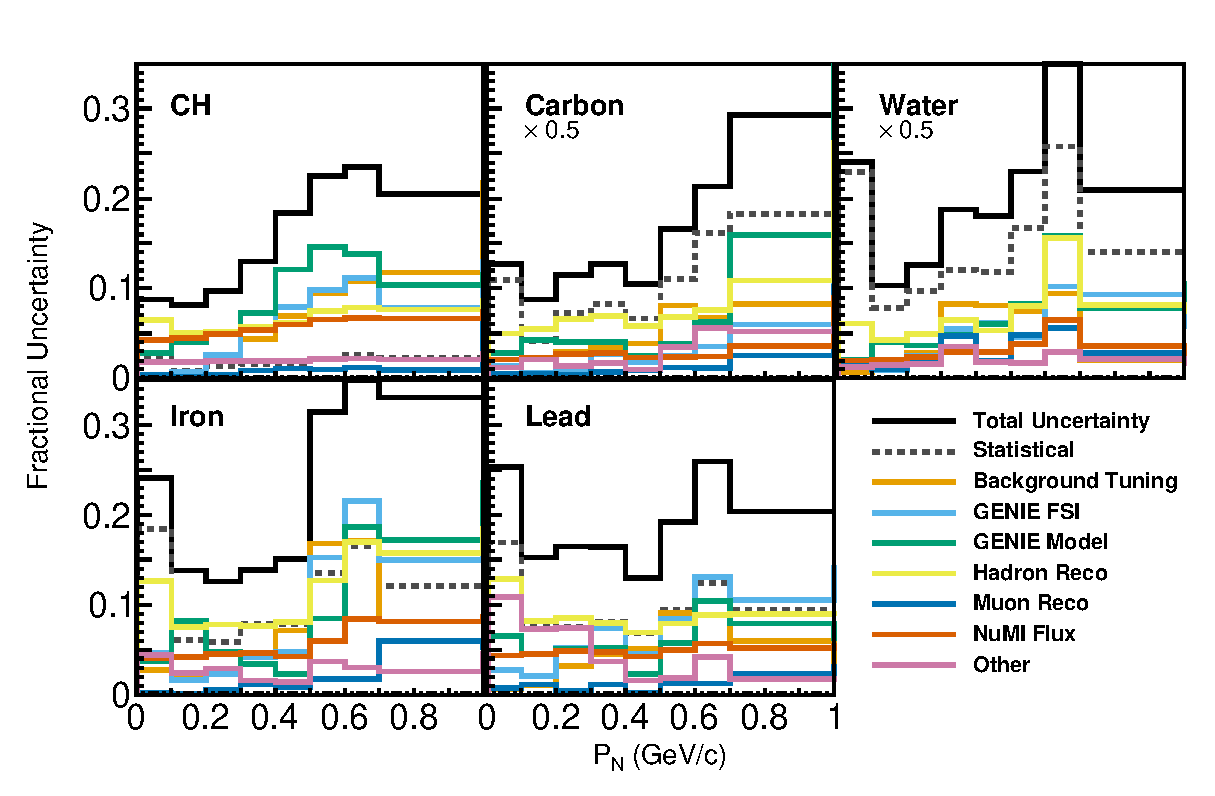
\includegraphics[width=\linewidth]{Figures/xsec_errors_all5/errors_pn.eps}
    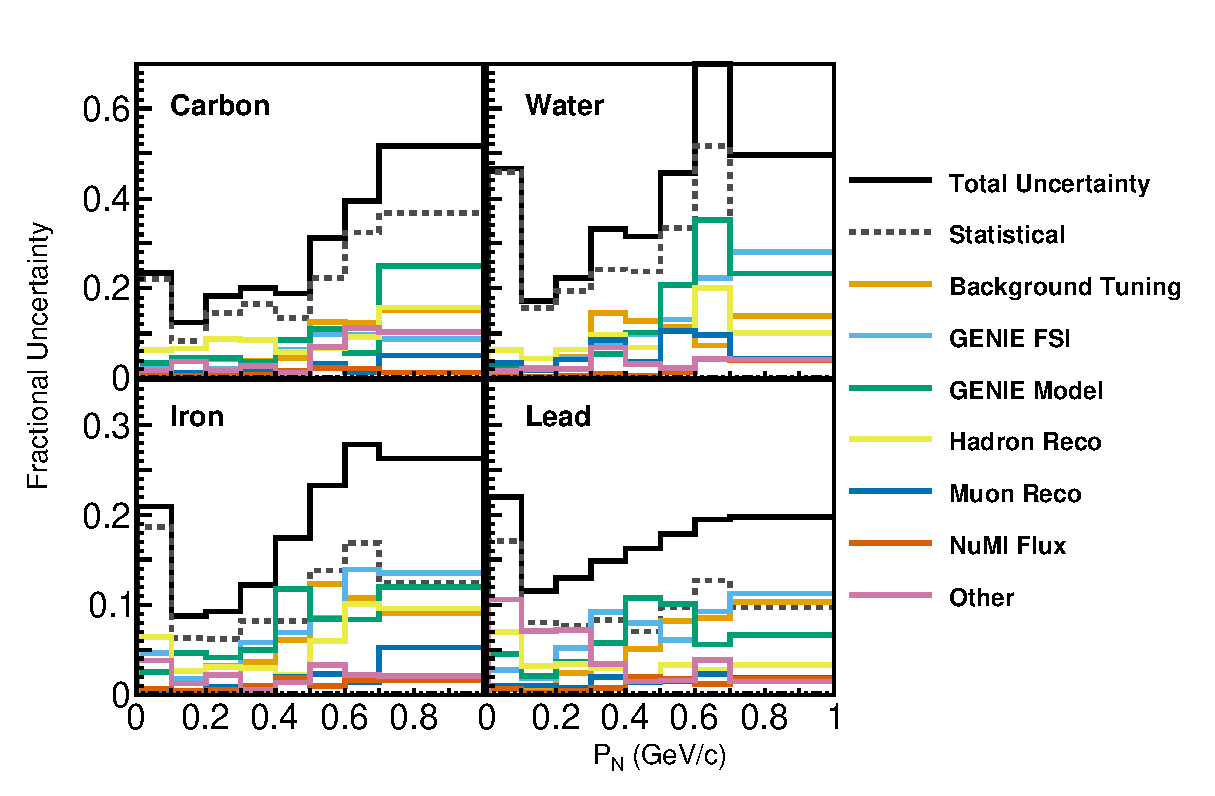
\includegraphics[width=\linewidth]{Figures/xsec_ratio_errors/ratio_errors_pn.eps}\caption[\tkipn cross-section ratio uncertainties for multiple targets]{Uncertainties on the absolute cross section for each target (upper five plots) and on the ratio to CH (lower four plots) as a function of \tkipn .}
    \label{fig:xsec_err_pn}
\end{figure}
% p_muon
\begin{figure}
	\centering
    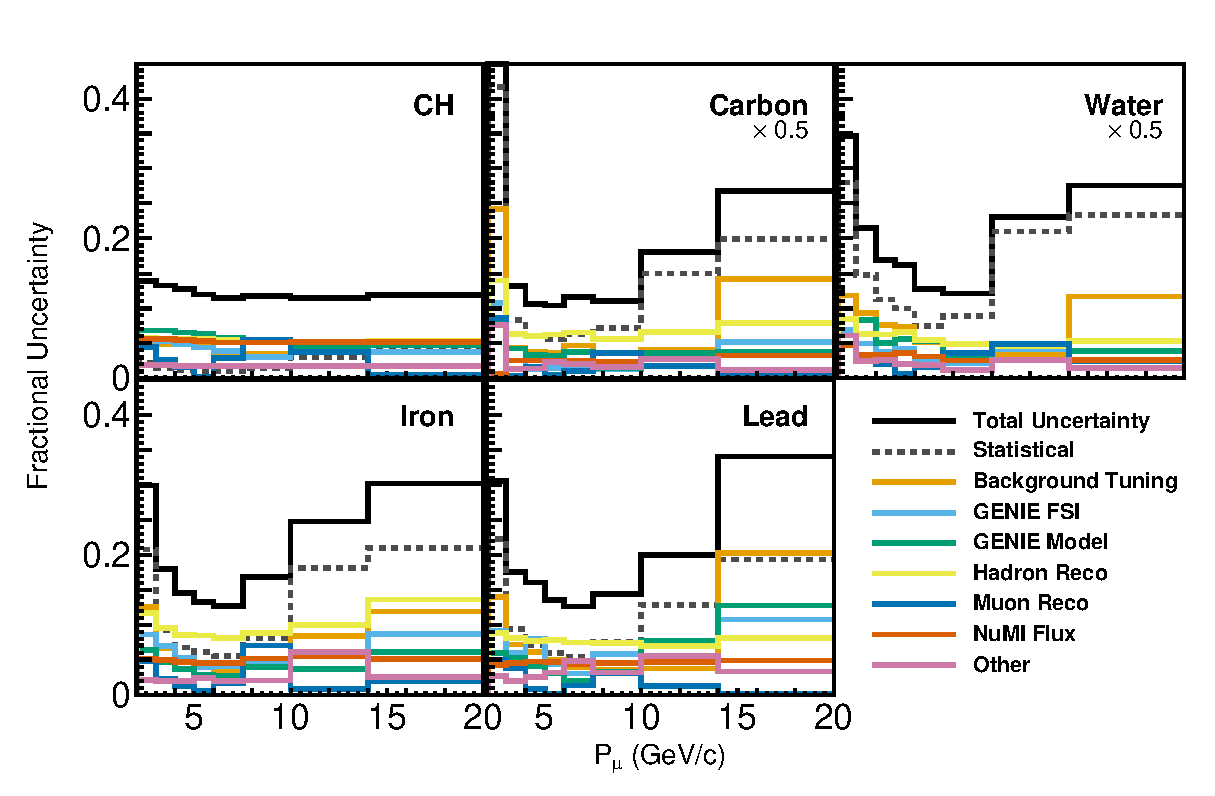
\includegraphics[width=\linewidth]{Figures/xsec_errors_all5/errors_muon_p.eps}
        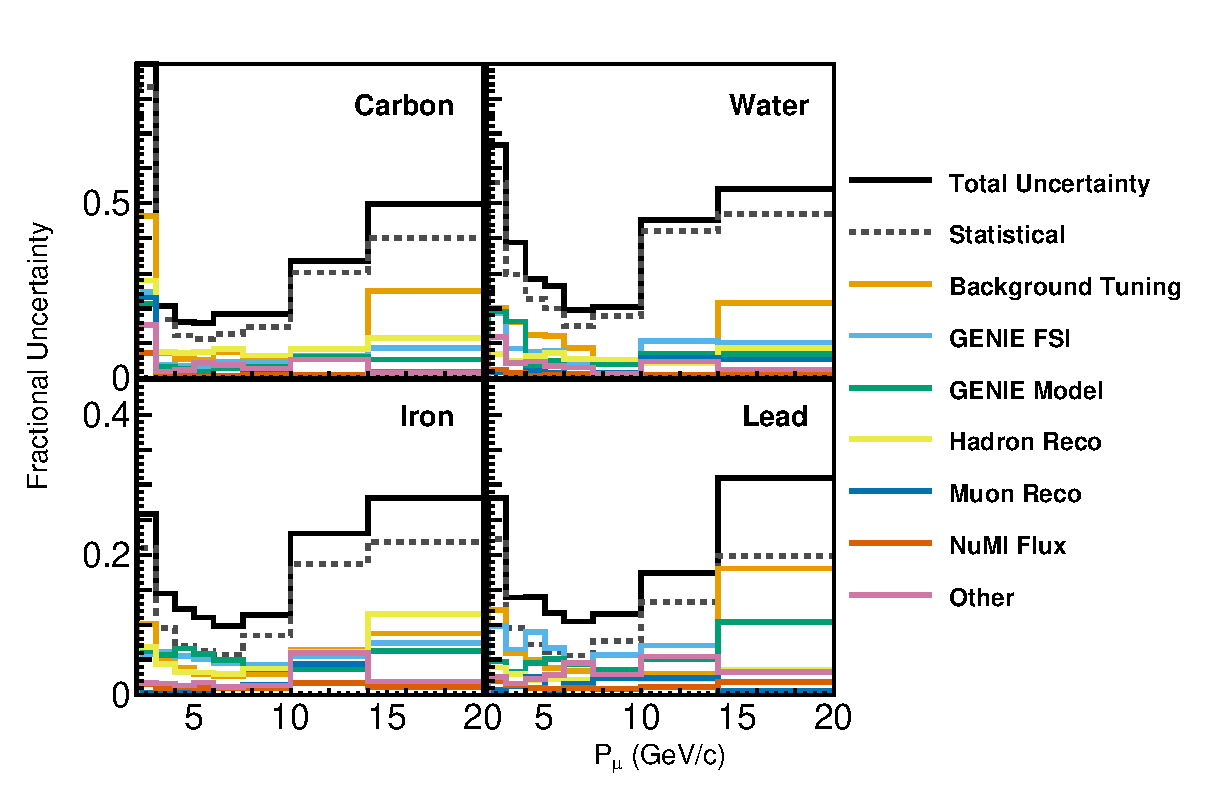
\includegraphics[width=\linewidth]{Figures/xsec_ratio_errors/ratio_errors_muon_p.eps}

    \caption[Muon momentum cross-section uncertainties for multiple targets ]{Uncertainties on the absolute cross section for each target (upper five plots) and on the ratio to CH (lower four plots) as a function of muon momentum.}
    \label{fig:xsec_err_muon_p}
\end{figure}
% pt_muon
\begin{figure}
	\centering
    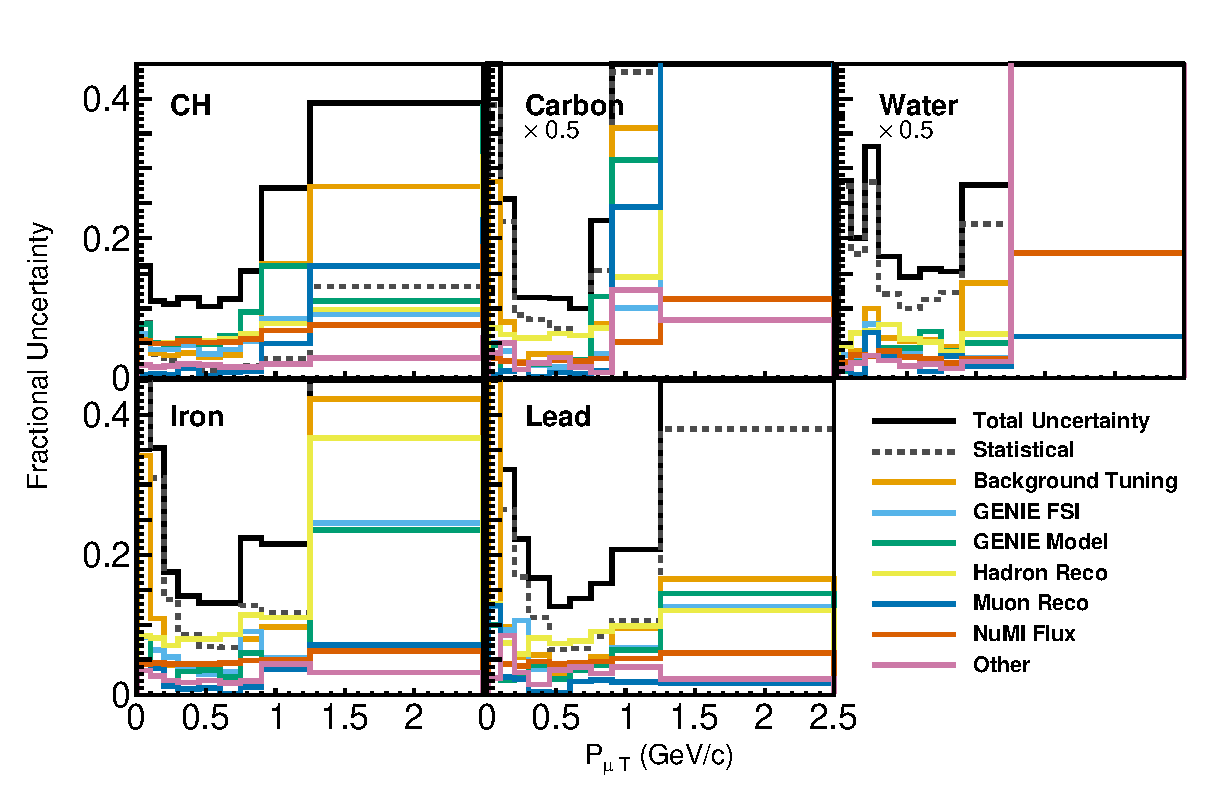
\includegraphics[width=\linewidth]{Figures/xsec_errors_all5/errors_muon_pt.eps}
        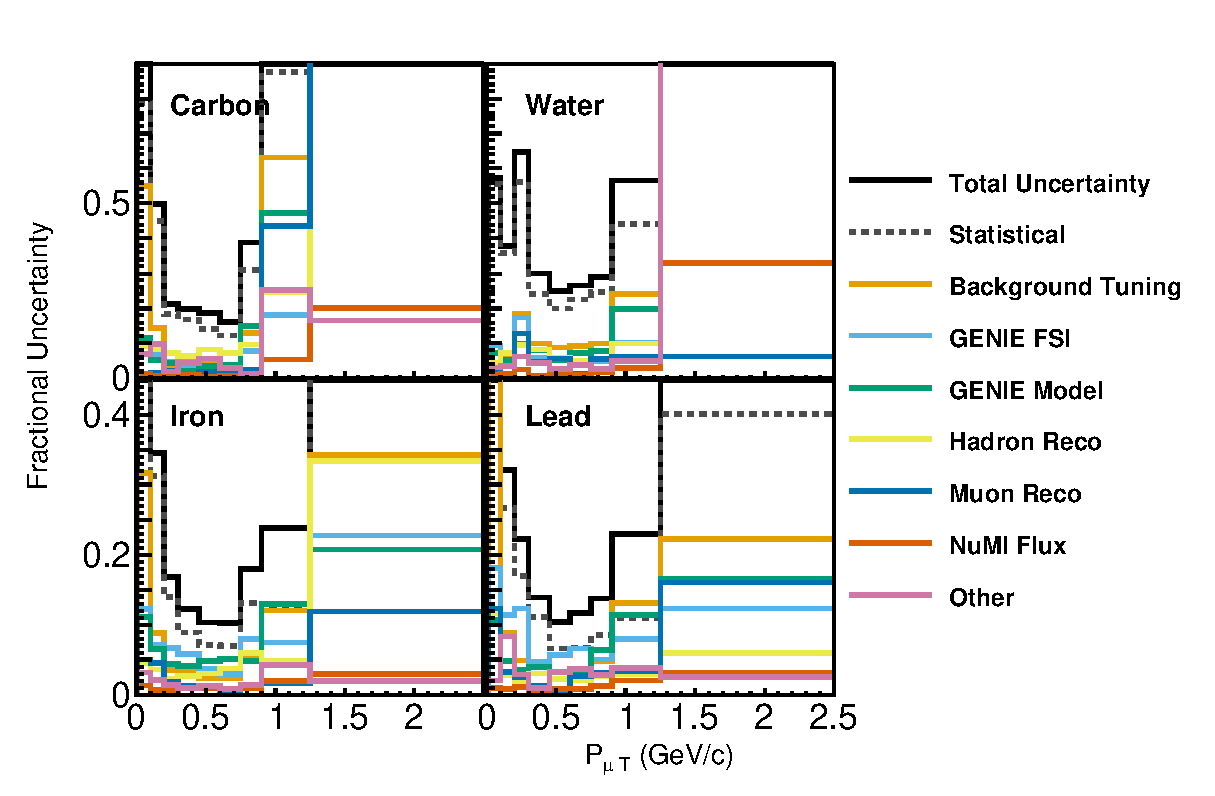
\includegraphics[width=\linewidth]{Figures/xsec_ratio_errors/ratio_errors_muon_pt.eps}
    \caption[Muon transverse momentum cross-section uncertainties for multiple targets]{Uncertainties on the absolute cross section for each target (upper five plots) and on the ratio to CH (lower four plots) as a function of muon transverse momentum.}
    \label{fig:xsec_err_muon_pt}
\end{figure}
% theta_muon
\begin{figure}
	\centering
    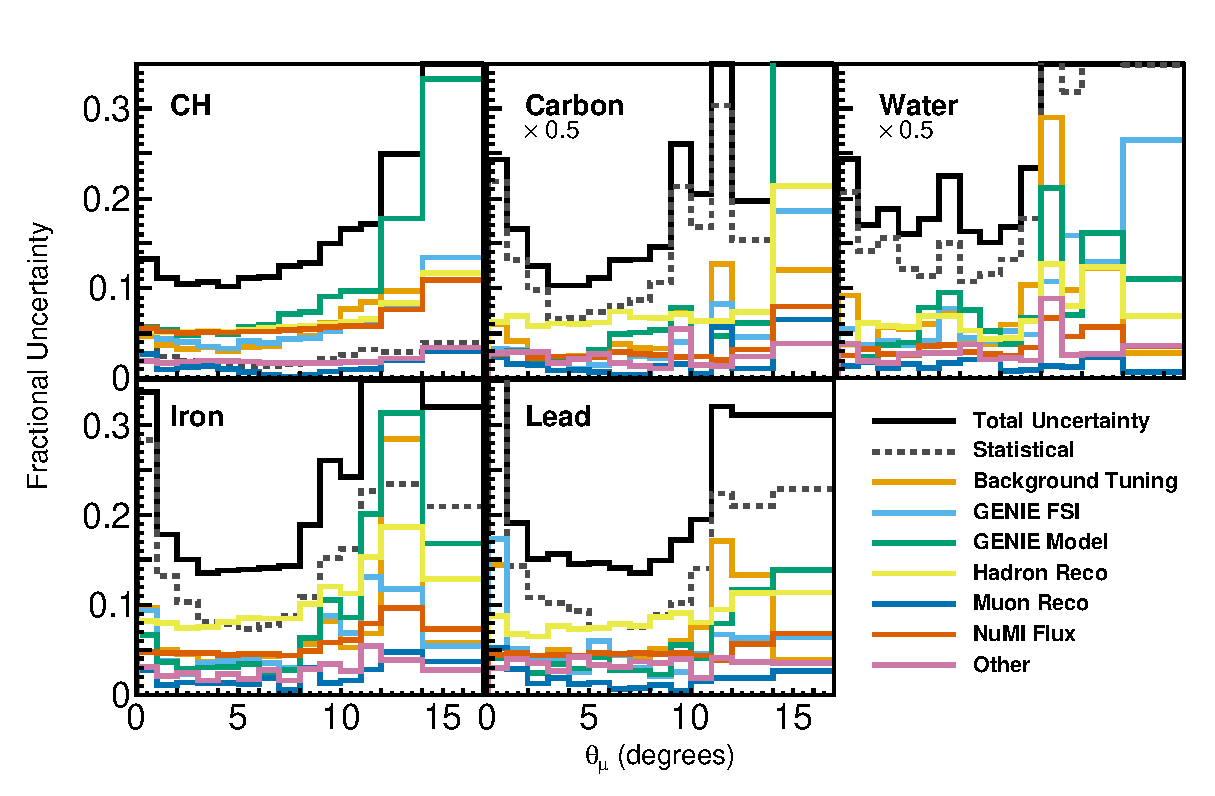
\includegraphics[width=\linewidth]{Figures/xsec_errors_all5/errors_muon_theta.eps}
    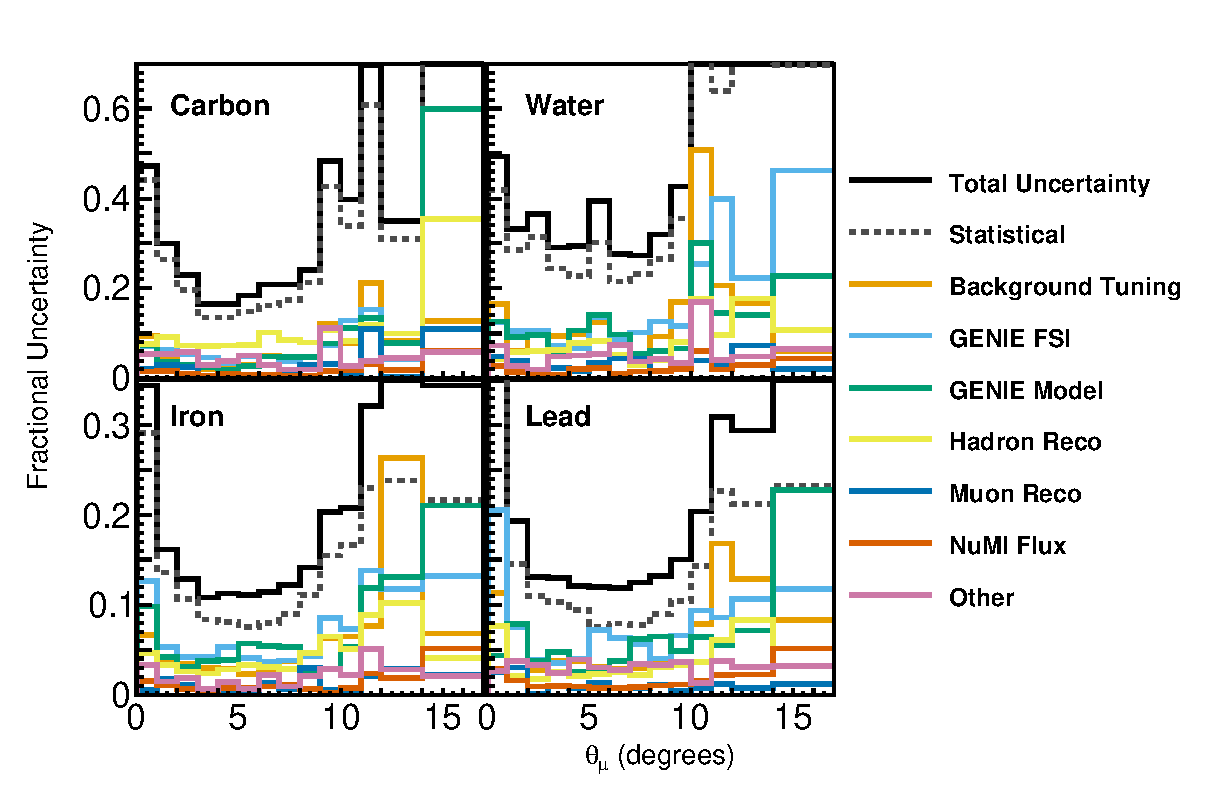
\includegraphics[width=\linewidth]{Figures/xsec_ratio_errors/ratio_errors_muon_theta.eps}
    \caption[$\theta_\mu$ cross-section uncertainties for multiple targets ]{Uncertainties on the absolute cross section for each target (upper five plots) and on the ratio to CH (lower four plots) as a function of $\theta_\mu$.}
    \label{fig:xsec_err_muon_theta}
\end{figure}
% p_proton
\begin{figure}
	\centering
    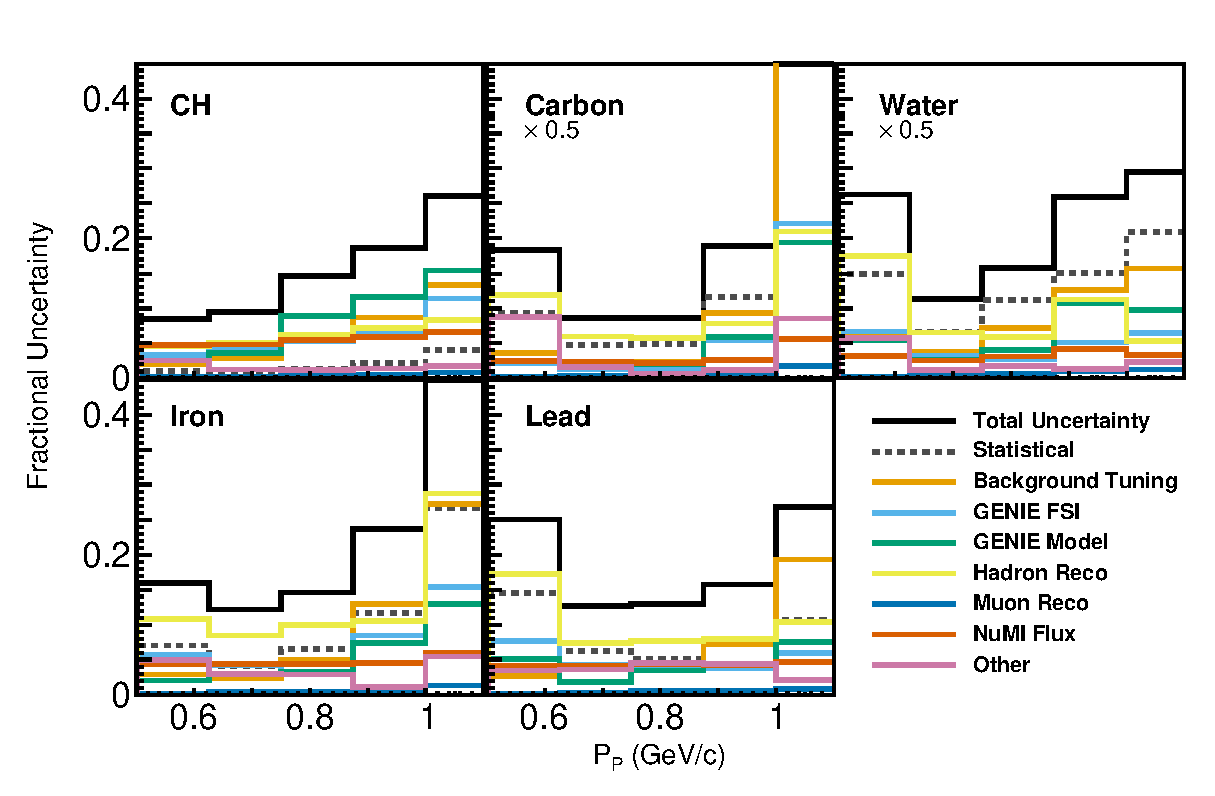
\includegraphics[width=\linewidth]{Figures/xsec_errors_all5/errors_proton_p.eps}
        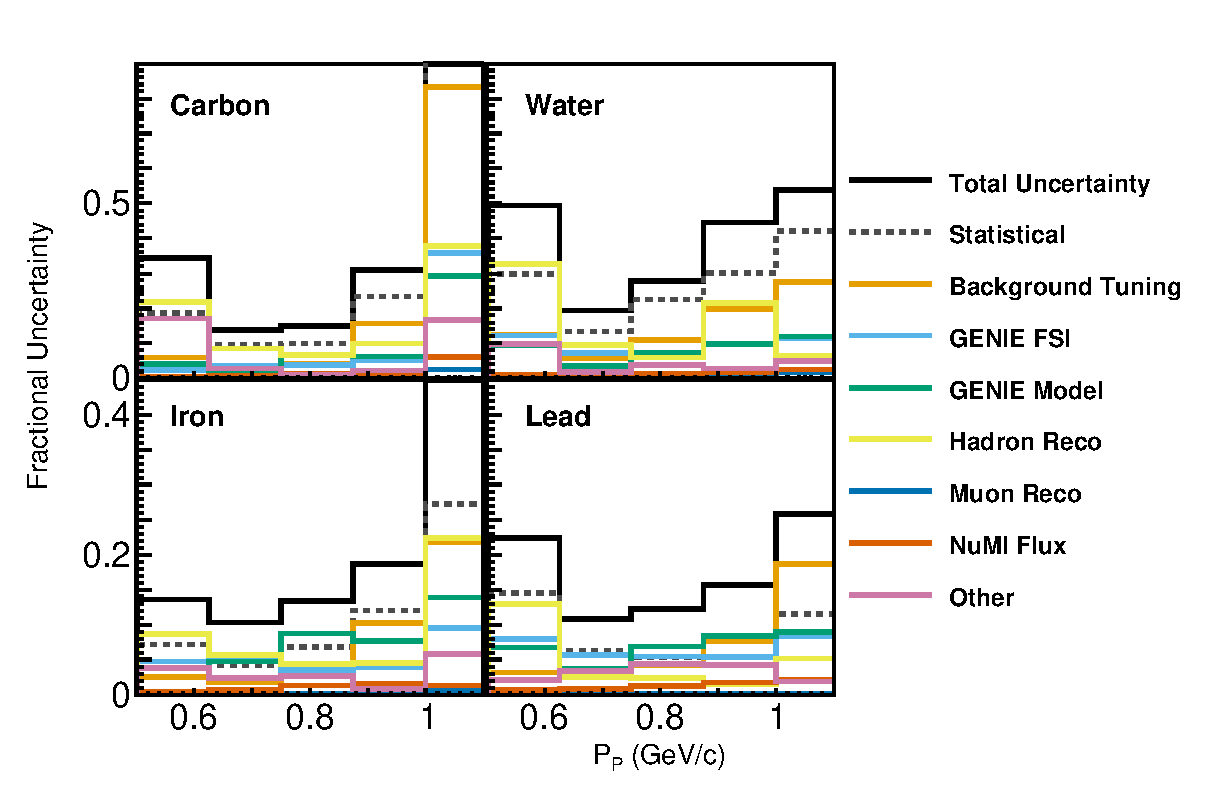
\includegraphics[width=\linewidth]{Figures/xsec_ratio_errors/ratio_errors_proton_p.eps}
    \caption[Proton momentum cross-section uncertainties for multiple targets ]{Uncertainties on the absolute cross section for each target (upper five plots) and on the ratio to CH (lower four plots) as a function of proton momentum.}
    \label{fig:xsec_err_proton_p}
\end{figure}
% pt_proton
\begin{figure}
	\centering
    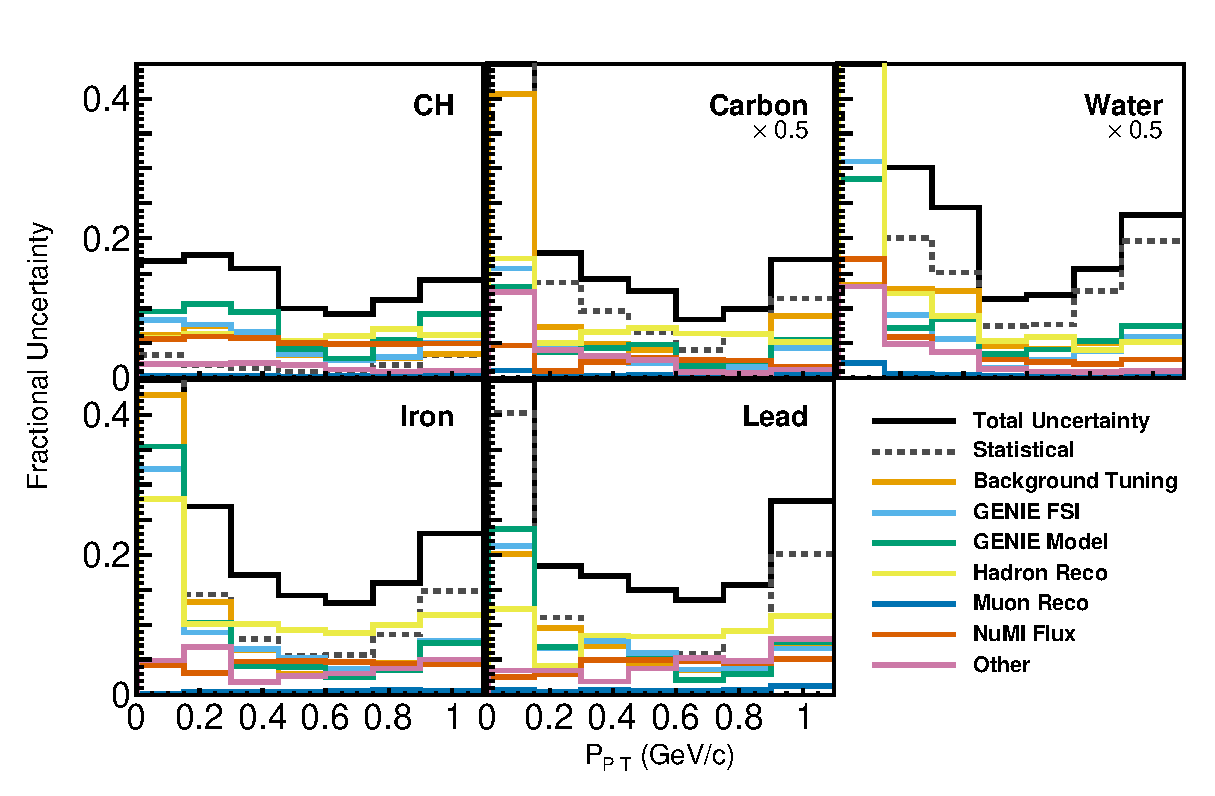
\includegraphics[width=\linewidth]{Figures/xsec_errors_all5/errors_proton_pt.eps}
        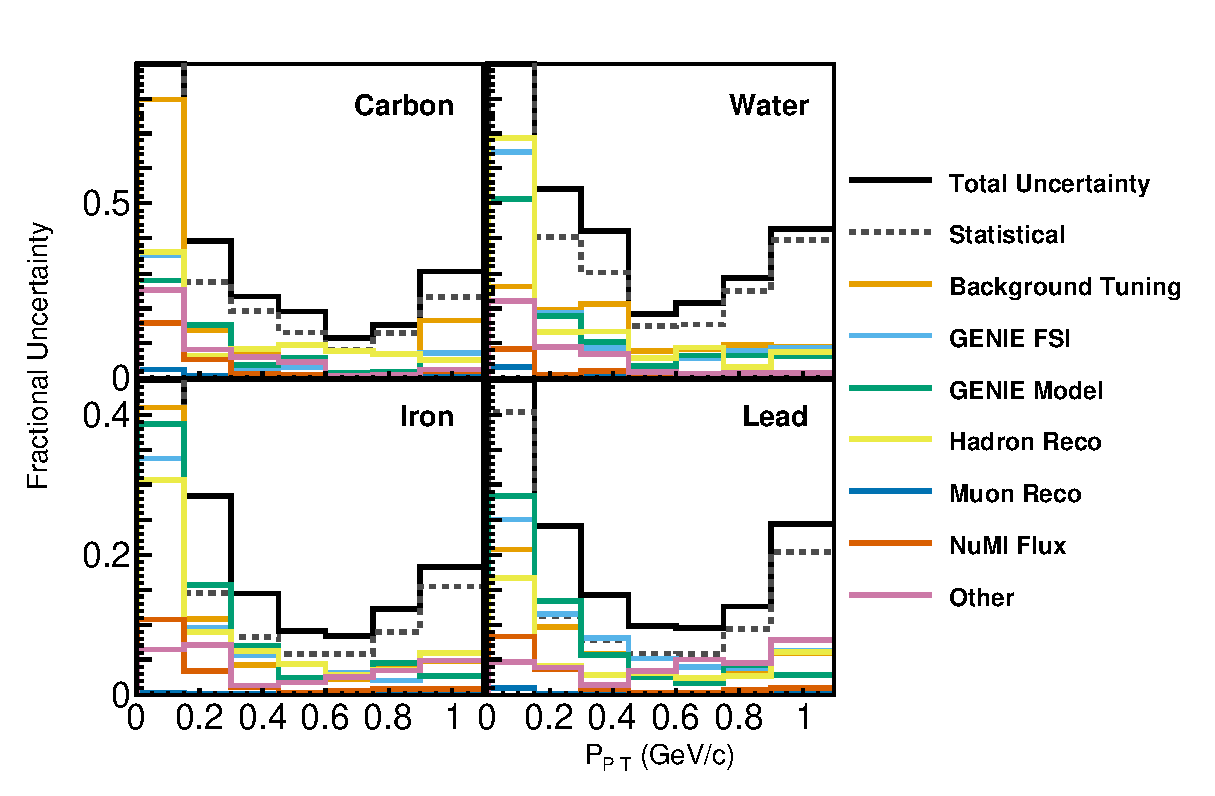
\includegraphics[width=\linewidth]{Figures/xsec_ratio_errors/ratio_errors_proton_pt.eps}
    \caption[cross-section uncertainties for multiple targets ]{Uncertainties on the absolute cross section for each target (upper five plots) and on the ratio to CH (lower four plots) as a function of proton transverse momentum.}
    \label{fig:xsec_err_proton_pt}
\end{figure}
% theta_proton
\begin{figure}
	\centering
    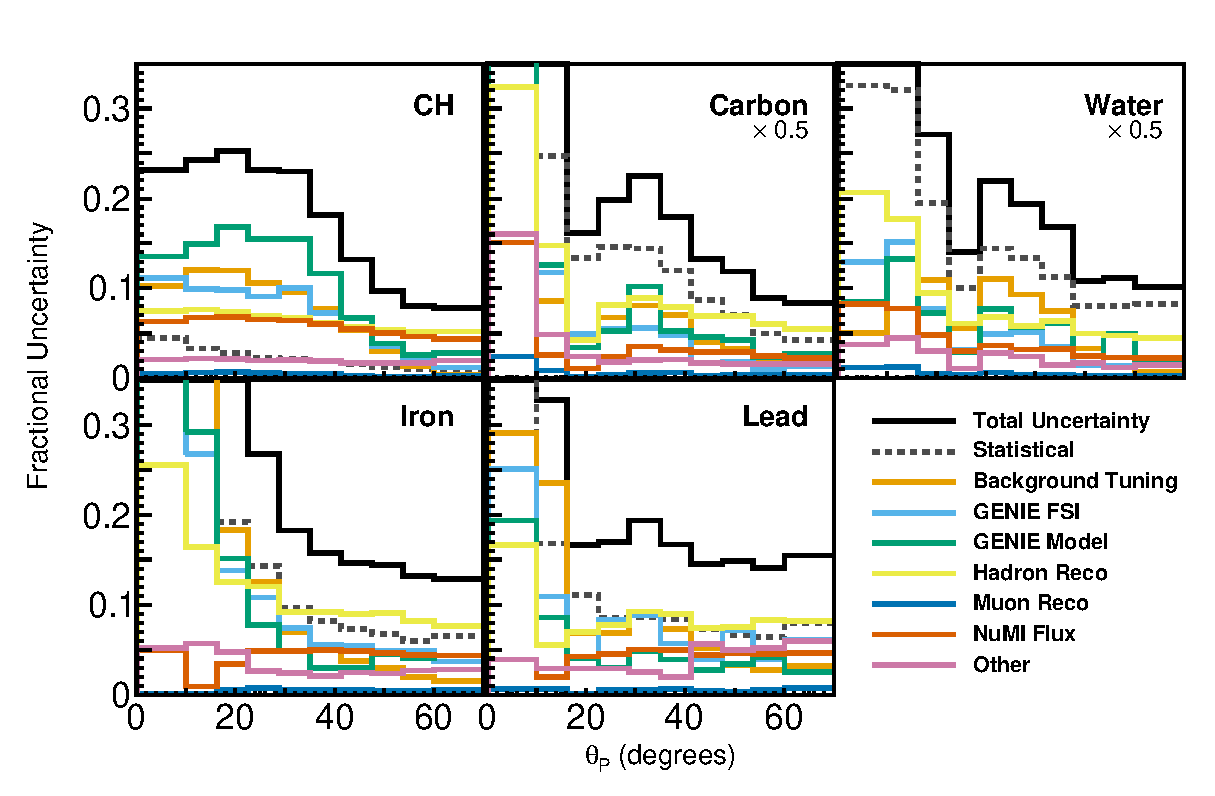
\includegraphics[width=\linewidth]{Figures/xsec_errors_all5/errors_proton_theta.eps}
    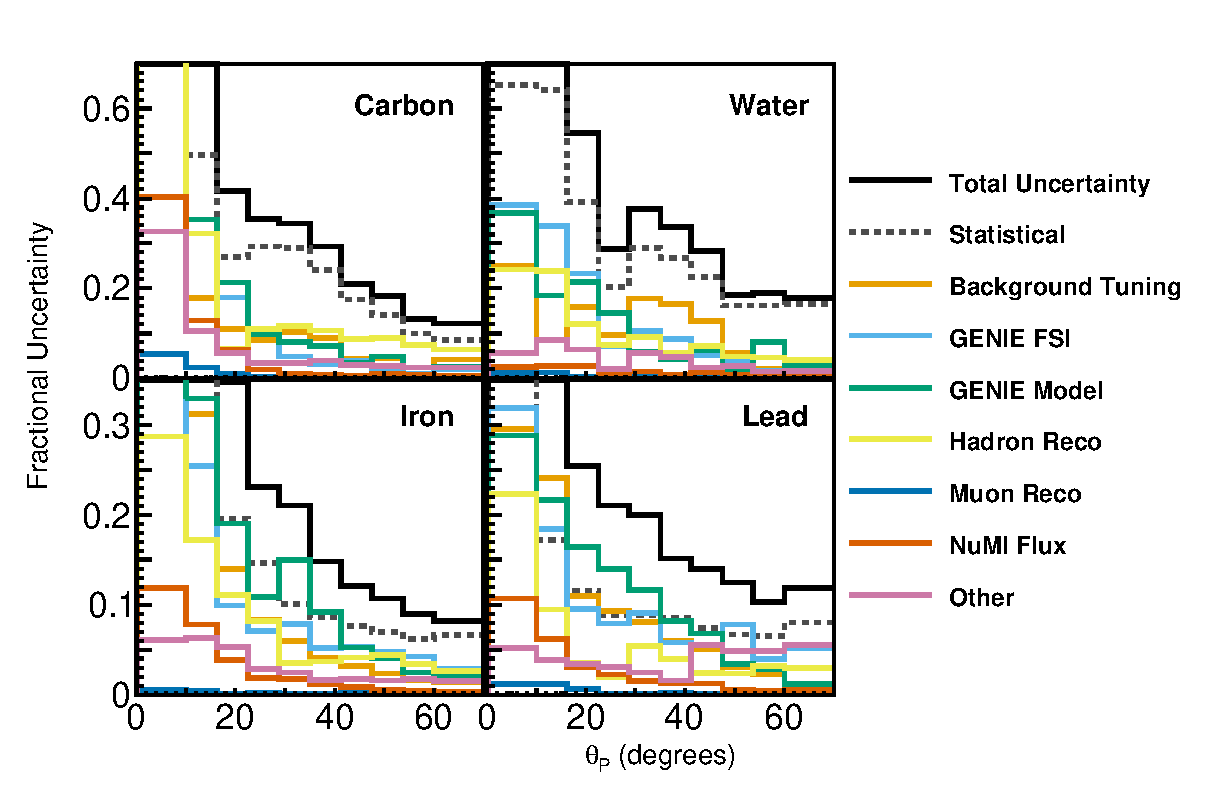
\includegraphics[width=\linewidth]{Figures/xsec_ratio_errors/ratio_errors_proton_theta.eps}
    \caption[$\theta_p$ cross-section uncertainties for multiple targets ]{Uncertainties on the absolute cross section for each target (upper five plots) and on the ratio to CH (lower four plots) as a function of proton angle with respect to the neutrino beam.}
    \label{fig:xsec_err_proton_theta}
\end{figure}